\sloppy
\documentclass[14pt,a4paper,oneside]{extarticle}	% Размер основного шрифта и формата листа
\usepackage{xltxtra}						% Используется для вывода логотипа XeLaTeX
\usepackage{xunicode}						% Кодировка документа
\usepackage{polyglossia}					% Загружает пакет многоязыковой верстки
\newfontfamily\russianfont{Book Antiqua}
%\setmainfont{Liberation Serif}						% Основной шрифт текста
\setmainfont{Book Antiqua}
\setdefaultlanguage{russian}				% Основной язык текста
\setotherlanguage{english}					% Дополнительный язык текста
\linespread{1}							% Межстрочный интервал выбран полуторным
\usepackage[left=2.5cm,
right=1.5cm,vmargin=2.5cm]{geometry} % Отступы по краям листа
\bibliographystyle{ugost2008}

\usepackage{xcolor}
\usepackage{hyperref}
% Цвета для гиперссылок
\definecolor{linkcolor}{HTML}{359B08} % цвет ссылок
\definecolor{urlcolor}{HTML}{799B03} % цвет гиперссылок
\hypersetup{pdfstartview=FitH,  linkcolor=linkcolor,urlcolor=urlcolor, colorlinks=true}

%---------------------------%
%---- Пакеты расширений ----%
%---------------------------%
\usepackage{xcolor}
\usepackage{hyperref}
% Цвета для гиперссылок
\definecolor{linkcolor}{HTML}{359B08} % цвет ссылок
\definecolor{urlcolor}{HTML}{799B03} % цвет гиперссылок
\hypersetup{pdfstartview=FitH,  linkcolor=linkcolor,urlcolor=urlcolor, colorlinks=true}


\usepackage{verbatim,indentfirst}
\usepackage{cite,enumerate,float}
\usepackage{amsmath,amssymb,amsthm,amsfonts}

%---------------------------%
%--- Вставка иллюстраций ---%
%---------------------------%
\usepackage{graphicx}
\usepackage{subfigure}
%\graphicspath{{Images/}}
\usepackage{fontspec}

\begin{document}
%	\pagestyle{empty} %  выключаенм нумерацию
	%\setcounter{page}{3}% Нумерация начинается с третьей страницы
	%\renewcommand{\contentsname}{\center{Содержание}}
	%\tableofcontents
	

	\begin{center}
		%\addcontentsline{toc}{section}{Потенциальный барьер}
		\subsection*{Потенциальный барьер}
	\end{center}
		

\begin{figure}[H] 	
	\centering 	
	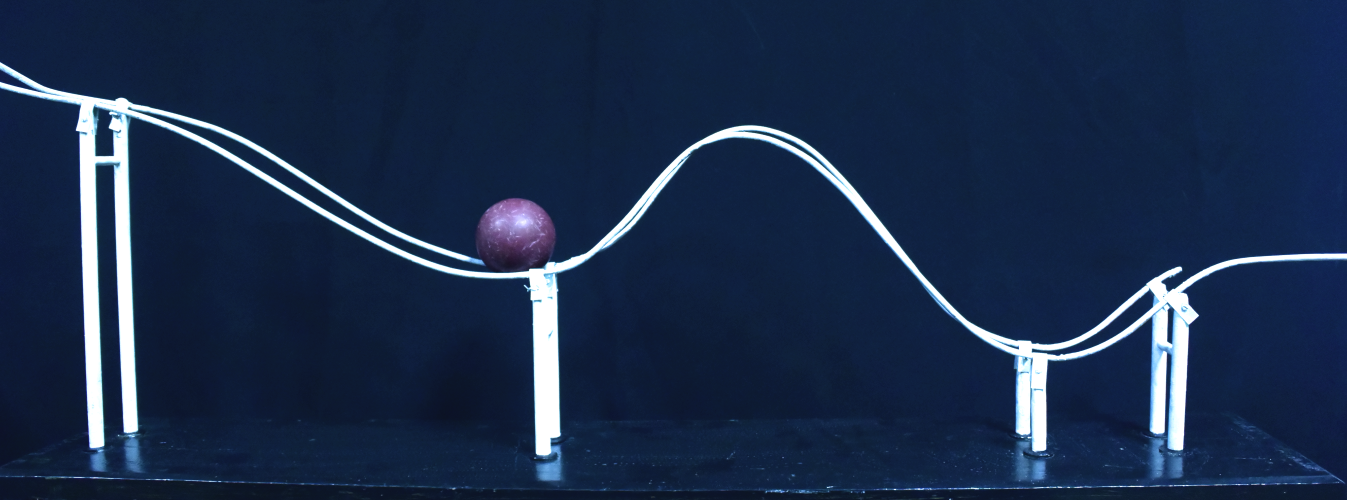
\includegraphics[width=0.9\linewidth]{barrier-1.png}
	\caption{Демонстрация особенностей движения механической системы в поле гравитационных сил}
	\label{barrier-1}
\end{figure}
	
	\subsection*{\underline{Оборудование:}}

		\begin{enumerate}
			\item Макет потенциального барьера в виде двух металлических направляющих.
			\item Массивный шар.
		\end{enumerate}
	
		\subsection*{\underline{Основные определения:}}
		
		Энергия есть универсальная мера количества любых видов движения материи.
		Состояние, в котором находится система тел, может быть определено заданием ряда величин.
		Величины, с помощью которых может быть полностью охарактеризовано состояние системы, называются параметрами.
		Поскольку энергия — мера движения, т.е. изменения состояния системы, то ее можно количественно выразить через параметры состояния, т.е. энергия есть функция состояния.
		
		В механике полная механическая энергия системы тел равна сумме кинетической энергии этих тел и потенциальной энергии их взаимодействия друг с другом
$$ W = E_{\text{к}} + E_{\text{п}}.$$

Кинетическая энергия зависит от скорости тел, а потенциальная энергия определяется взаимным расположением (зависит от координат) частей системы.

	\subsection*{\underline{Краткое описание:}}
 
Можно проследить за движением шара (рис.\ref{barrier-2}), поднятого до наивысшей точки на горке.
После того, как шар отпускают, он начинает катиться вниз под действием силы тяжести.
Если на его пути окажется горка меньшей высоты, то шару удастся преодолеть этот барьер. 

Если же отпустить шар с меньшей высоты, то его скорости окажется недостаточно для преодоления барьера. 
В следствие чего, поднявшийся на некоторую высоту шар после полной остановки начинается двигаться в обратную сторону.
После того, как он поднимается на горку, по которой он был отпущен в первый раз, его движение вновь повторится.
Такой периодически повторяющийся процесс подъема и опускания обусловлен наличием в системе точки минимума потенциальной энергии.
Шар, попадая в так называемую потенциальную яму оказывается неспособным преодолеть потенциальный барьер (горку), если запас его энергии оказывается недостаточным.

В условиях демонстрации величина потенциальной энергии прямо пропорциональна высоте шара над поверхностью земли.
Поэтому при запуске шара с высоты, больше чем высота горки (начальная потенциальная энергия в этом случае больше энергии потенциального барьера) его энергии оказывается достаточно для преодоления барьера.
При движении шара с высоты равной или меньшей, чем высота барьера, ему не удается преодолеть эту горку.
При таком колебательном движении шара внутри потенциальной ямы, ограниченной двумя потенциальными барьерам, можно заметить, что шар на протяжении всего времени движения не достигнет своей начальной высоты.
Постепенное уменьшение энергии происходит в результате присутствия силы трения между направляющими и шаром.

\newpage
\subsection*{\underline{Теория:}}
	
Закон сохранения энергии позволяет провести анализ общих закономерностей движения, если известна зависимость потенциальной энергии от координат. 
Рассмотрим движение материальной частицы, вдоль оси $ x $ в потенциальном поле, показанном на рис.\ref{barrier-2}.
Поскольку в однородном поле сил тяжести потенциальная энергия пропорциональна высоте подъема тела, то распределение потенциальной энергии можно представить в виде функции $ E_{\text{п}}(x) $, соответствующей профилю горки, обозначенной синим цветом на рис.\ref{barrier-2}. Участок $ NPQ $ — является потенциальной ямой, а $ QLF $ — потенциальным барьером.

Из закона сохранения энергии $  W = E_{\text{к}} + E_{\text{п}}  $ и из того условия, что кинетическая энергия $ E_{\text{к}} = W - E_{\text{п}} $ всегда положительна, следует, что частица может находиться лишь в областях, где $ E_{\text{п}} < W $.
На схеме частица с энергией $ W = E_{1\text{п}} $, находящаяся в точке $ N $, способна двигаться только внутри области $ NPQ $ и ее энергии оказывается недостаточно для преодоления потенциального барьера $ QLF $.
Начиная движение из точки $ M $ с потенциальной энергией $ E_{2\text{п}} > E_{1\text{п}} $ частица может оказаться в области за потенциальным барьером.
\begin{figure}[H] 	
	\centering 	
	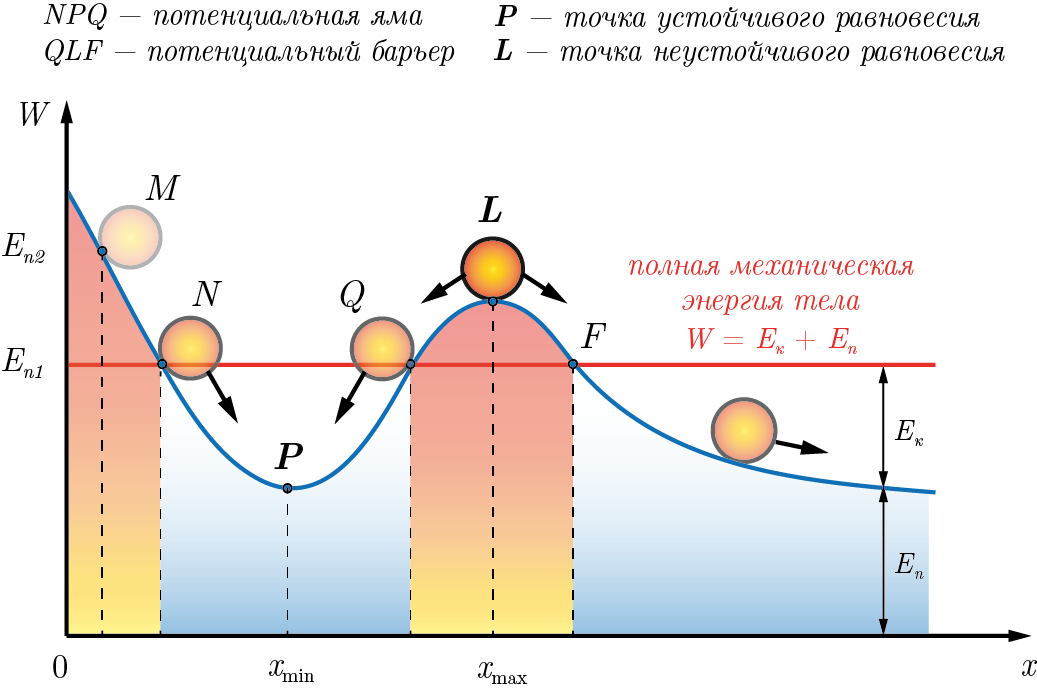
\includegraphics[width=0.95\linewidth]{barrier-2.png}
	\caption{Движение частицы вблизи положений устойчивого и неустойчивого равновесия (потенциальная яма и потенциальный барьер на кривой). Синий цвет обозначает график потенциальной энергии, красный -- полной энергии}
	\label{barrier-2}
\end{figure}

В первом случае ее движение будет ограничено (финитно), в точке $ Q $ произойдет полная остановка и направление движения частицы изменится на противоположное.
Такой процесс в теории будет происходит бесконечно долго, если в системе пренебречь силами трения и диссипацией энергии.
Во второй области движение частицы будет не ограниченным (инфинитным): преодолев потенциальный барьер она способна удалиться бесконечно далеко от начала координат направо.

В точках экстремума потенциальной энергии $ x_{min} $ и $ x_{max} $ сила, действующая на частицу, равна нулю, потому что равна нулю производная потенциальной энергии:
\begin{equation}\label{barrier-1eq1}
F_{x} = -\frac{d W}{d x} = 0.
\end{equation}

Точка $ P $ в этом случае будет называться положение устойчивого равновесия, а точка $ L $ — неустойчивого. 
Частица может испытывать небольшие отклонения (флуктуации) от положения равновесия.
При этом в точке устойчивого равновесия возникают силы, которые возвращают частицу к положению равновесия. 
При малом отклонении частицы в точке неустойчивого равновесия возникающие силы еще дальше «уводят» ее от начального положения.

Попробуем показать, что описанные выше положения равновесия существуют.
Для тела в точке экстремума (далее $ x_{min} $ и $ x_{max} $ обозначим через $ x_{m} $) действующая на него сила равна нулю $ F_{x} = 0 $.

Пусть вследствие малого возмущения координата частицы изменяется на небольшую величину $ \Delta x $. 
При таком изменении координаты на частицу начнет действовать сила:
\begin{equation}\label{barrier-1eq2}
F_{x}(x_{m} + \Delta x) = F_{x}(x_{m}) + \Delta x \frac{d F_{x}}{d x}(x_{m})
\end{equation}

С учетом выражения (\ref{barrier-1eq1}), имеем:
\begin{equation}\label{barrier-1eq3}
F_{x}(x_{m} + \Delta x) \approx - \Delta x \frac{d^{2} W_{x}}{d x^{2}}(x_{m})
\end{equation}

В точке \textbf{P} с минимумом энергии вторая производная потенциальной энергии положительна: $$ \frac{d^{2} W_{x_{min}}}{d x^{2}} > 0.$$
Поэтому при положительных отклонениях от положения равновесия ($ x > 0 $) возвращающая сила $ F $ отрицательна, а при $ x<0 $ — положительна.
В обоих случаях сила оказывается противоположно смещению частицы, из-за чего положение равновесия вблизи точки с минимумом потенциальной энергии оказывается устойчиво.

Обратная ситуация наблюдается в положении \textbf{L} c наибольшей энергией, так как в этом случае вторая производная потенциальной энергии по координате оказывается отрицательной: $$ \frac{\partial^{2} W_{x_{max}}}{\partial x^{2}} < 0. $$ 
В результате смещение частицы  $ \Delta x $ приводит к возникновению положительной силы $ F $, которая в свою очередь только увеличивает смещение частицы из положения равновесия. 
Такое положение равновесия оказывается неустойчивым.
\end{document}
